\documentclass[a4paper,11pt]{article}
\usepackage{ls}
%\usepgfplotslibrary{patchplots}
\pgfplotsset{compat=newest} 

\pagestyle{empty}
\begin{document}

\begin{center}
  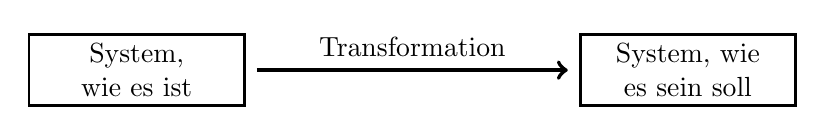
\begin{tikzpicture}[line width=1pt,
      pfeil/.style={shorten <=4pt, shorten >=4pt, line width=1.5pt},
      mytext/.style={text width=2.5cm,align=center}]
    \node[draw,mytext] at (0,0) [rectangle] (A0) {System, wie es ist};
    \node[draw,mytext] at (7,0) [rectangle] (A2) {System, wie es sein soll};
    \draw[pfeil,->] (A0)--(A2) ;
    \node[fill=white] at (3.5,.3) [rectangle] {Transformation};
  \end{tikzpicture}
\end{center}
\end{document}

\begin{center}
  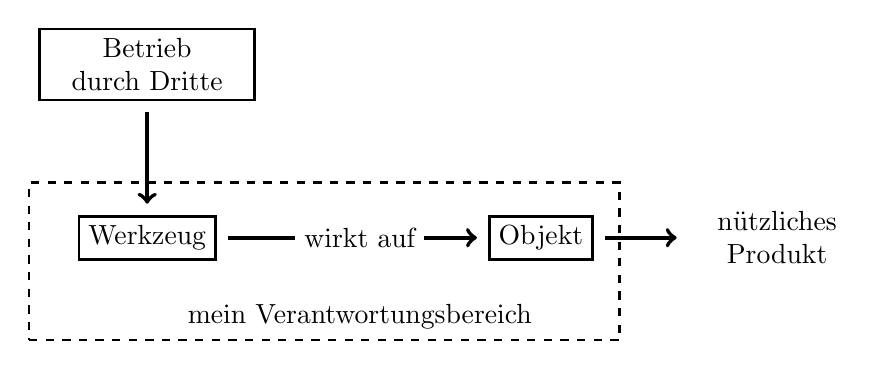
\begin{tikzpicture}[line width=1pt,
      pfeil/.style={shorten <=4pt, shorten >=4pt, line width=1.5pt},
      mytext/.style={text width=2.5cm,align=center}]
    \node[draw] at (0,1.3) [rectangle] (A0) {Werkzeug};
    \node[draw] at (5,1.3) [rectangle] (A2) {Objekt};
    \node[text width=2cm,align=center] at (8,1.3) [rectangle] (A3) {nützliches Produkt};
    \node[draw,mytext] at (0,3.5) [rectangle] (A4) {Betrieb durch Dritte};
    %\node[mytext,below of = A0] {Old state of the library};
    %\node[mytext,below of = A1] {New state of the library};
    \draw[pfeil,->] (A0)--(A2) ;
    \draw[pfeil,->] (A2)--(A3) ;
    \draw[pfeil,->] (A4)--(A0) ;
    \draw[dashed] (-1.5,0) -- (6,0) -- (6,2) -- (-1.5,2) -- cycle ;
    \node[fill=white] at (2.7,1.3) [rectangle] {wirkt auf};
    \node[] at (2.7,.3) {mein Verantwortungsbereich};
  \end{tikzpicture}
\end{center}
\end{document}

\begin{center}
  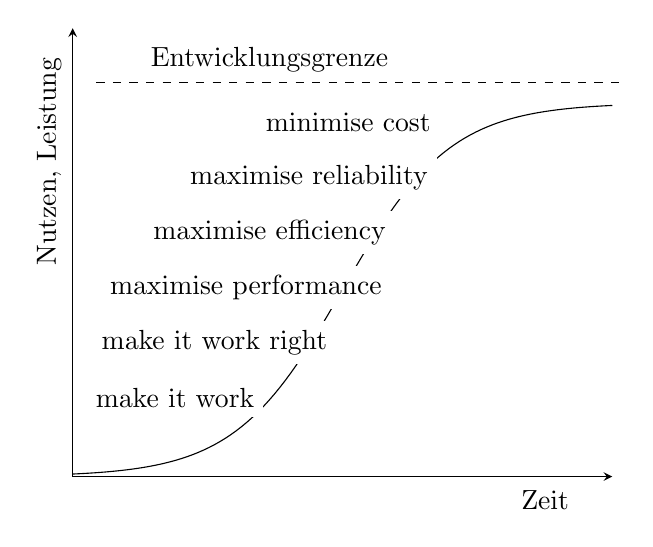
\begin{tikzpicture}
    \begin{axis}[
        xmin=0, xmax=10, ymin=0,ymax=12,
        axis lines=middle,
        xtick={\empty},ytick={\empty},
      ]
      \addplot[samples=100,domain=0:10] expression {10/(1+exp(-(x-5))) } ;
    \end{axis}
    \node[rotate=90] at (-.3,4) {Nutzen, Leistung} ;
    \node[] at (6,-.3) {Zeit} ;
    \node[] at (2.5,5.3) {Entwicklungsgrenze}; 
    \draw[-,dashed] (0.3,5) -- (7,5) ;
    \node[fill=white] at (1.3,1) {make it work} ;
    \node[fill=white] at (1.8,1.7) {make it work right} ;
    \node[fill=white] at (2.2,2.4) {maximise performance} ;
    \node[fill=white] at (2.5,3.1) {maximise efficiency} ;
    \node[fill=white] at (3,3.8) {maximise reliability} ;
    \node[fill=white] at (3.5,4.5) {minimise cost} ;
  \end{tikzpicture}\\[1em]
  Entwicklungsschritte entlang der S-Kurve am Beispiel Verbrennungsmotor
\end{center}
\end{document}
